\documentclass{llncs}
\usepackage{fullpage}

%load needed packages
\usepackage{graphicx}
\usepackage{array}
\usepackage{booktabs}
\usepackage[utf8]{inputenc}
\usepackage{amsmath} 


\begin{document}

\title{APPLICATION OF CLUSTERING METHODS TO
	SPORULATION YEAST MICROARRAY DATA}

\author{Diego De Pablo}
\institute{\email{depablodiego@uma.es} \\
Health Engineering. Málaga University.}

\maketitle 

\vspace{1cm} % Space down the title

\textit{This work presents a comparison between three main clustering methods applied to yeast sporulation data: K-means, hierarchical clustering and self-organizing maps (SOM). K-means was used to cluster genes based on expression patterns, selecting the optimal number of clusters using the elbow method. Hierarchical clustering allowed to analyze the structure of the data without predefining a number of clusters, using a dendrogram to identify significant groups. Finally, SOM was applied as an unsupervised clustering technique, with a visual representation reflecting the topology of the data. This comparison aims to evaluate the effectiveness of each method in gene clustering, similar to the work Comparisons and validation of statistical clustering techniques for microarray gene expression data}

% This is a comment


\section{Introduction}


The aim of this study is to apply clustering techniques to a DNA microarray dataset of \textit{Saccharomyces cerevisiae} gene expression during sporulation, and compare the results with those from a separate analysis.


\subsection*{Temporal Patterns in Gene Expression During Sporulation}

Gene expression during sporulation follows distinct temporal patterns, observe the figure \ref{fig:Sporlutation}, reflecting specific cellular events \cite{chu1998}. These include:
\begin{itemize}
	\item \textbf{Metabolic Early:} Rapid induction at t0.
	\item \textbf{Early I and II:} Sustained expression from t0.5 to t2.
	\item \textbf{Early-Middle:} Peak expression around t5.
	\item \textbf{Middle:} Activation between t5 and t7, related to meiosis.
	\item \textbf{Mid-Late:} Increased expression from t7 to t9, linked to spore wall formation.
	\item \textbf{Late:} Induction between t9 and t11.5, associated with spore maturation.
\end{itemize}
\vspace{-25pt}

\begin{figure}[h!]
	\begin{center}  % Usamos el entorno 'center'
		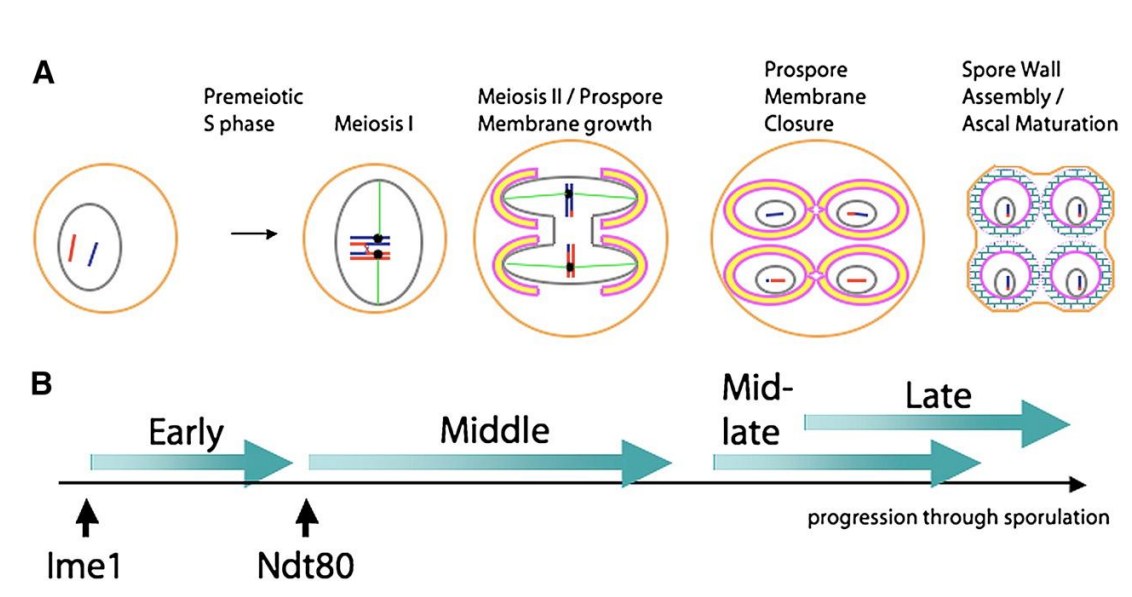
\includegraphics[width=0.55\textwidth]{images/sporlutation.png}
		\caption{A representation of the process of sporulation in budding yeasts}
		\label{fig:Sporlutation}
	\end{center}
\end{figure}


By utilizing DNA microarrays encompassing a significant portion of key genes, we can comprehensively investigate temporal gene expression patterns throughout the process of meiotic spore formation. However, this technique generates large datasets of unlabeled gene expression data, making pattern identification challenging. The abundance of expression levels for hundreds of genes at different time points presents an ideal scenario for applying clustering algorithms to uncover meaningful gene groups and understand the underlying transcriptional regulatory mechanisms.\cite{datta2003}

\subsection*{Application of Clustering Techniques to Analyze Sporulation Data}

While hierarchical clustering (UPGMA) with correlation distance has been a popular choice in microarray studies (at least the begginnings of this century), it's important to recognize the diverse range of clustering algorithms available in pattern recognition and statistics. To classify genes based on their temporal expression profiles during yeast sporulation, we will employ various clustering algorithms, including hierarchical clustering, K-means, self-organizing maps (SOM), and Diana. This comparative analysis aims to identify distinct gene expression patterns and gain insights into the underlying transcriptional regulatory mechanisms.\cite{datta2003}



\section{description of the methods}

There is a wide variety of clustering techniques, in this work it was decided to focus on details that were not carried out in the paper Comparisons and validation of statistical
clustering techniques for microarray gene
expression data by the Datta brothers, giving priority to the following:
\subsection{clustering techniques}


\begin{itemize}
	\item \textbf{Hierarchical Clustering with Correlation:} Hierarchical clustering with correlation is a method that groups data into a hierarchical structure rather than assigning a fixed number of clusters beforehand. It starts with each data point as a separate cluster and gradually merges the closest clusters until a single cluster remains.\cite{guess2002}
	
	\begin{itemize}
		\item \textbf{Algorithm:} The "average" method is used to calculate the distance between clusters. This method computes the average distance between points in one cluster and points in the other cluster.\cite{datta2003}
		
		\item \textbf{Common Method:} This approach, known as UPGMA, is a popular and straightforward method for hierarchical clustering.\cite{datta2003}
		
		\item \textbf{Distance Metric:} The distance between genes is calculated using a correlation-based measure, where a higher correlation indicates greater similarity between the gene expression profiles.\cite{datta2003}
	\end{itemize}
	
	
		
		\item \textbf{K-means Clustering:} Clustering is an unsupervised machine learning technique used to divide a dataset into distinct groups or clusters. Each cluster consists of data points that are more similar to each other than to those in other clusters. K-means is a popular clustering algorithm that partitions data into a predefined number of clusters, represented by centroids. The algorithm works iteratively to assign data points to the nearest centroid, updating centroids based on the mean of the points assigned to each cluster.\cite{steinley2006}
		
		\begin{enumerate}
			\item \textbf{Initialization:} k points are randomly selected from the dataset as initial centroids of the k clusters. These centroids represent the center of each cluster.
			\item \textbf{Assigning Points to Clusters:} Each data point is assigned to the cluster whose centroid is closest. The distance is usually calculated using the Euclidean distance.
			\item \textbf{Updating Centroids:} The positions of the centroids are recalculated as the average of all the points assigned to each cluster.
			\item \textbf{Repetition:} Steps 2 and 3 are repeated until the centroids no longer move significantly or a maximum number of iterations is reached.\cite{steinley2006}
		\end{enumerate}
		
		\item \textbf{Self-Organizing Maps (SOM):} is an unsupervised neural network that learns to map high-dimensional data onto a low-dimensional grid. It identifies representative prototype vectors and establishes a continuous mapping from the input space to this grid. The grid, often visualized as a 2D map (see Figure \ref{fig:som}), consists of neurons with associated weight vectors. These weight vectors are initially random but converge to represent clusters of similar data points during training.
		
	
\end{itemize}

\begin{figure}[h!]
	\begin{center}  % Usamos el entorno 'center'
		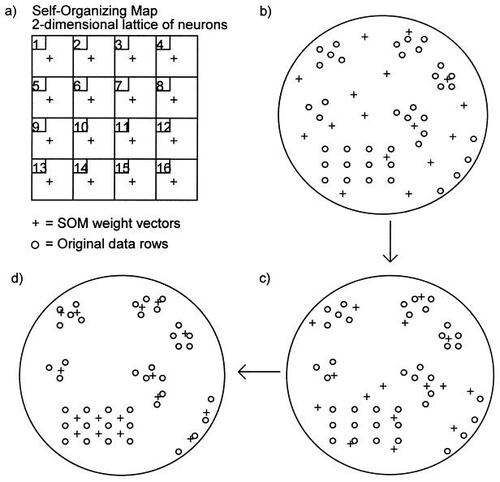
\includegraphics[width=0.45\textwidth]{images/som.jpg}
		\caption{The image illustrates the Self-Organizing Map (SOM) learning process. Panel (a) shows the initial SOM structure, (b) depicts the random initialization of weight vectors, (c) represents an intermediate stage of learning, and (d) shows the final configuration where weight vectors cluster around data points.}
		\label{fig:som}
	\end{center}
\end{figure}

\vspace{-30pt}

\subsection{Additional Clustering Methods which are theoretically mentioned}

\begin{itemize}
	\item \textbf{DIANA (Divisive Analysis Clustering):} This method differs from hierarchical clustering in that it starts with all data in a single cluster and progressively divides it into sub-clusters.\cite{datta2003}
	
	\item \textbf{Fanny:} Utilizes fuzzy logic to generate a probability vector for each observation, assigning observations to clusters based on the highest probability. L1 distance (Manhattan distance) is typically used as the dissimilarity measure, offering robustness compared to Euclidean distance. \cite{datta2003}
	
	\item \textbf{Model-based Clustering:} Treats the data as arising from a mixture of distributions, allowing for a probabilistic interpretation of clusters.\cite{datta2003}
	
	\item \textbf{Hierarchical Clustering with Partial Least Squares:} Leverages partial least squares to identify gene relationships through their expression profiles, demonstrating its effectiveness as noted by Datta (2001)\cite{datta2003}.
\end{itemize}

\subsection{Validation Methods}


To validate the obtained clusters, we can employ various strategies. One approach is to experiment with different numbers of clusters and observe how the average distance between points and their respective cluster centroids changes. This is known as the \textit{elbow method} due to the characteristic elbow shape of the resulting graph. However, the elbow method alone does not guarantee optimal cluster formation.\cite{Wang2018Thresher}

\subsubsection{Silhuoette}

To address this, we can utilize \textit{silhouette analysis}, a cluster validation technique based on the silhouette coefficient. The silhouette coefficient measures the similarity of a data point to its own cluster compared to its similarity to neighboring clusters. It ranges from -1 to 1, with values closer to 1 indicating better cluster membership and values closer to -1 suggesting misclassification.\cite{Wang2018Thresher}


In simple terms, it helps us determine whether the data has been grouped correctly and whether the clusters formed are coherent.
The silhouette coefficient is calculated as follows:

\begin{itemize}
	\item \(a\): The average distance between a point and all other points in its cluster. This tells us how well the point fits within its cluster.
	\item \(b\): The average distance between a point and all points in the nearest different cluster.This tells us how well the point would fit into the closest neighboring cluster.
\end{itemize}

\[
\text{Silhouette Coefficient} = \frac{(b - a)}{\max(a, b)}
\]

By calculating the average silhouette coefficient for all points within each cluster, we can assess the overall cluster validity. Combining silhouette analysis with the elbow method can help us determine the optimal number of clusters that minimize the overall distance between points and their clusters while maximizing the silhouette coefficient, suggesting well-formed and meaningful clusters.\cite{Wang2018Thresher}

\subsubsection{Calinski-Harabasz Index}


The Calinski-Harabasz Index (CHI) is a metric used to assess the quality of clustering in cluster analysis, offering a different approach from the silhouette coefficient. It evaluates the clustering performance by comparing two types of sum of squares:\cite{Ning2023Clustering}

\begin{itemize}
	\item \textbf{Between-cluster sum of squares (SSB):} Measures the separation between the cluster centroids. A higher SSB indicates that clusters are more distinct from each other.
	\item \textbf{Within-cluster sum of squares (SSW):} Measures the dispersion of data points within each cluster. A lower SSW indicates that the clusters are more compact.
\end{itemize}

The Calinski-Harabasz Index is calculated using the following formula:

\[
\text{CHI} = \frac{\text{SSB} / (k - 1)}{\text{SSW} / (n - k)}
\]

where:
\begin{itemize}
	\item $k$ is the number of clusters.
	\item $n$ is the total number of data points.
\end{itemize}

A higher CHI value indicates better clustering quality, as it suggests that clusters are well separated and the data within each cluster are homogeneous. Thus, the index provides a measure of the balance between cluster separation and the compactness of the data points within each cluster.\cite{Ning2023Clustering}

\subsubsection{The Davies-Bouldin Index}

 is a widely used metric for evaluating the quality of clustering, offering an approach that complements other measures such as the silhouette coefficient and the Calinski-Harabasz index. It provides an assessment of whether the formed clusters are both compact and well-separated. The index is calculated as the average similarity between each cluster and its most similar neighboring cluster, with lower values indicating better clustering performance.\cite{Davies1979Cluster}

\subsubsection*{Calculation of the Davies-Bouldin Index}

The computation of the DBI involves several steps:

\begin{enumerate}
	\item \textbf{Centroid Calculation:} For each cluster, compute the centroid, which is the average of all data points within the cluster.
	\item \textbf{Cluster Diameter Calculation:} For each cluster, calculate its diameter, defined as the maximum distance between any two points in the cluster.
	\item \textbf{Centroid Distance Calculation:} Calculate the distance between the centroids of each pair of clusters.
	\item \textbf{Similarity Calculation:} For each cluster, find the nearest neighboring cluster (the one with the closest centroid) and compute the similarity using the formula:
	\[
	S(i) = \frac{D(i) + D(j)}{d_{ij}}
	\]
	where:
	\begin{itemize}
		\item $S(i)$ is the similarity of cluster $i$ to its nearest neighbor $j$.
		\item $D(i)$ and $D(j)$ are the diameters of clusters $i$ and $j$, respectively.
		\item $d_{ij}$ is the distance between the centroids of clusters $i$ and $j$.
	\end{itemize}
\end{enumerate}

The Davies-Bouldin Index is then computed as the average of the similarity values for all clusters.\cite{Davies1979Cluster}

In essence, the Davies-Bouldin Index seeks to minimize the similarity between clusters, with lower values reflecting better-defined and more compact clusters.

\subsubsection{Average Proportion of Non-Overlap Measure} It is a metric used by the Datta brothers in Comparisons and validation of statistical clustering techniques for microarray gene expression data\cite{datta2003}, denoted as $V_1$, is used to evaluate the consistency of a clustering algorithm by examining the stability of gene assignments across different clustering scenarios. It is defined as:

\[
V_1 = \frac{1}{M l} \sum_{g=1}^{M} \sum_{i=1}^{l} \left( 1 - \frac{n(C_{g,i} \cap C_{g,0})}{n(C_{g,0})} \right),
\]

where:
\begin{itemize}
	\item $M$ is the total number of genes.
	\item $l$ is the number of time points.
	\item $C_{g,0}$ represents the cluster assignment of gene $g$ when using the full dataset.
	\item $C_{g,i}$ represents the cluster assignment of gene $g$ when the expression levels at time point $T_i$ are excluded.
	\item $n(C_{g,i} \cap C_{g,0})$ is the number of genes that remain in the same cluster in both the original and reduced datasets.
\end{itemize}

The measure calculates the average proportion of genes that are not assigned to the same cluster when comparing the clustering results obtained using the complete dataset with the results obtained after removing expression data for one time point. Lower values of $V_1$ indicate greater stability and consistency of the clustering algorithm, reflecting better preservation of gene cluster assignments despite variations in the data.\cite{datta2003}


\section{most relevant results obtained comparing both methods}

\textbf{Bold paragraph. Lorem ipsum dolor sit amet, consectetur adipiscing elit, sed do eiusmod tempor incididunt ut labore et dolore magna aliqua. Ut enim ad minim veniam, quis nostrud exercitation ullamco laboris nisi ut aliquip ex ea commodo consequat. Duis aute irure dolor in reprehenderit in voluptate velit esse cillum dolore eu fugiat nulla pariatur. Excepteur sint occaecat cupidatat non proident, sunt in culpa qui officia deserunt mollit anim id est laborum.}
 
 
 \section{Conclusions}
 
 \textbf{Bold paragraph. Lorem ipsum dolor sit amet, consectetur adipiscing elit, sed do eiusmod tempor incididunt ut labore et dolore magna aliqua. Ut enim ad minim veniam, quis nostrud exercitation ullamco laboris nisi ut aliquip ex ea commodo consequat. Duis aute irure dolor in reprehenderit in voluptate velit esse cillum dolore eu fugiat nulla pariatur. Excepteur sint occaecat cupidatat non proident, sunt in culpa qui officia deserunt mollit anim id est laborum.}

\bibliographystyle{plain}  % Puedes cambiar "plain" por el estilo de tu preferencia, como apalike, ieeetr, etc.
\bibliography{bibliography}  % Aquí va el nombre de tu archivo .bib (sin la extensión .bib)
\end{document}
